\documentclass{beamer}

%\usepackage[table]{xcolor}
\mode<presentation> {
  \usetheme{Boadilla}
%  \usetheme{Pittsburgh}
%\usefonttheme[2]{sans}
\renewcommand{\familydefault}{cmss}
%\usepackage{lmodern}
%\usepackage[T1]{fontenc}
%\usepackage{palatino}
%\usepackage{cmbright}
  \setbeamercovered{transparent}
\useinnertheme{rectangles}
}
%\usepackage{normalem}{ulem}
%\usepackage{colortbl, textcomp}
\setbeamercolor{normal text}{fg = black}
\setbeamercolor{structure}{fg = blue}
\definecolor{trial}{cmyk}{1,0,0, 0}
\definecolor{trial2}{cmyk}{0.00,0,1, 0}
\definecolor{darkgreen}{rgb}{0,.4, 0.1}
\definecolor{mygray}{gray}{0.8}
\definecolor{myblack}{rgb}{0, 0, 0}
\usepackage{array}
\beamertemplatesolidbackgroundcolor{white}  \setbeamercolor{alerted
text}{fg=red}

\setbeamertemplate{caption}[numbered]\newcounter{mylastframe}

\usepackage{color}
\usepackage{tikz}
\usetikzlibrary{arrows}
\usepackage{colortbl}
\usepackage{graphicx}

%\usepackage[usenames, dvipsnames]{color}
%\setbeamertemplate{caption}[numbered]\newcounter{mylastframe}c
%\newcolumntype{Y}{\columncolor[cmyk]{0, 0, 1, 0}\raggedright}
%\newcolumntype{C}{\columncolor[cmyk]{1, 0, 0, 0}\raggedright}
%\newcolumntype{G}{\columncolor[rgb]{0, 1, 0}\raggedright}
%\newcolumntype{R}{\columncolor[rgb]{1, 0, 0}\raggedright}

%\begin{beamerboxesrounded}[upper=uppercol,lower=lowercol,shadow=true]{Block}
%$A = B$.
%\end{beamerboxesrounded}}
\renewcommand{\familydefault}{cmss}
%\usepackage[all]{xy}

\usepackage{tikz}
\usepackage{lipsum}

 \newenvironment{changemargin}[3]{%
 \begin{list}{}{%
 \setlength{\topsep}{0pt}%
 \setlength{\leftmargin}{#1}%
 \setlength{\rightmargin}{#2}%
 \setlength{\topmargin}{#3}%
 \setlength{\listparindent}{\parindent}%
 \setlength{\itemindent}{\parindent}%
 \setlength{\parsep}{\parskip}%
 }%
\item[]}{\end{list}}
\usetikzlibrary{arrows}
%\usepackage{palatino}
%\usepackage{eulervm}
\usecolortheme{lily}

\newtheorem{com}{Comment}
\newtheorem{lem} {Lemma}
\newtheorem{prop}{Proposition}
\newtheorem{thm}{Theorem}
\newtheorem{defn}{Definition}
\newtheorem{cor}{Corollary}
\newtheorem{obs}{Observation}
 \numberwithin{equation}{section}


\title[PLSC 43401] % (optional, nur bei langen Titeln nötig)
{Mathematical Foundations of Political Methodology}

\author{Robert Gulotty}
\institute[University of Chicago]{Associate Professor\\Department of Political Science \\  University of Chicago}
\vspace{0.3in}
\date{August 28th, 2017}

\setbeamertemplate{navigation symbols}{}

\begin{document}



\begin{frame}
\titlepage
\end{frame}



\begin{frame}

\begin{itemize}
\item \textcolor{myblack}{Derivative}
\item \textcolor{myblack}{Derivative and Continuity}
\item \textcolor{myblack}{Derivative Rules}
\item \textcolor{myblack}{Mean Value Theorem}
\item \textcolor{myblack}{Second Derivatives}
\end{itemize}

\end{frame}



\begin{frame}

\begin{itemize}
\item \textcolor{myblack}{Derivative}
\item \textcolor{mygray}{Derivative and Continuity}
\item \textcolor{mygray}{Derivative Rules}
\item \textcolor{mygray}{Mean Value Theorem}
\item \textcolor{mygray}{Second Derivatives}
\end{itemize}

\end{frame}



\begin{frame}
\frametitle{Derivative: Motivation}

\begin{itemize}
\item[-] Derivatives describe the rates of change in functions \pause
\item[-] Foundational across a lot of work in Political Science. \pause
\item[-] A special limit \pause
\item[-] In this lecture, we will cover three broad ideas \pause
\begin{itemize}
\item[-] Geometric interpretation/intuition \pause
\item[-] Formulas/Algebra derivatives \pause
\item[-] Famous theorems
\end{itemize}
\end{itemize}

\end{frame}



\begin{frame}
\frametitle{Line and Slope}

\ \\A line can be represented by the equation $y=a*x+b$, with $a$ being the slope and $b$ the $y-$intercept \pause

\ \\For any points on the line, $(x_{o}, y_{o})$ and $(x_{1}, y_{1})$, we have $a = \frac{y_{1} - y_{o}}{x_{1} - x_{o}}$


\begin{center}
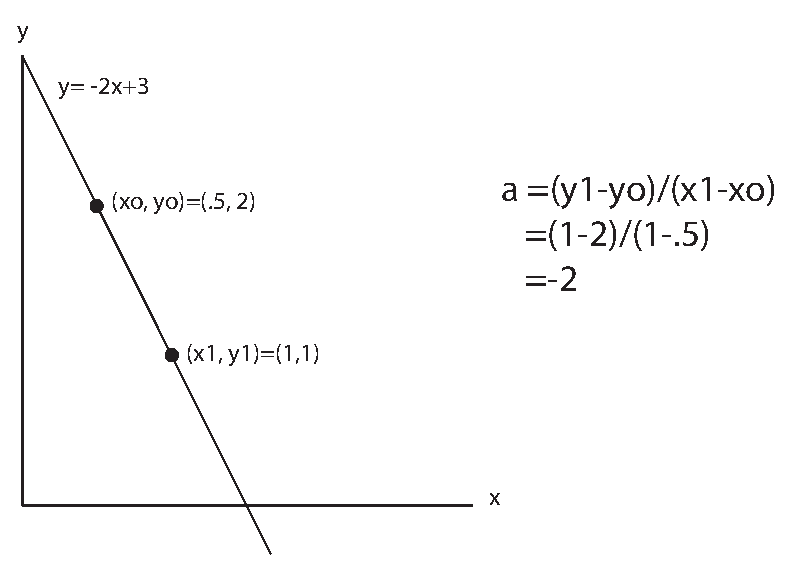
\includegraphics[scale = 0.5]{slope.eps}
\end{center}

\end{frame}



\begin{frame}
\frametitle{Slope of a Curve}

The slope of a curve, $f(x)$, at point $P$ is the limit of the slope of the line between $Q$ and $P$ as $Q\rightarrow P$

\begin{center}
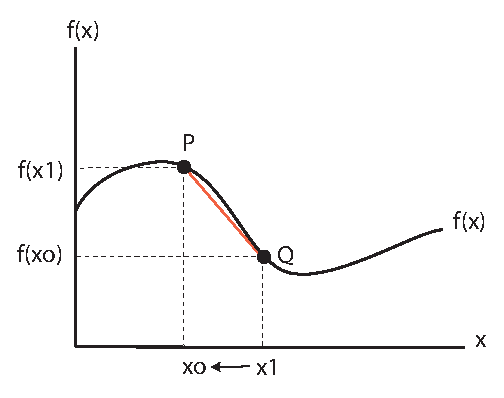
\includegraphics[scale = 0.5]{slopeCurve.eps}
\end{center}

\end{frame}



\begin{frame}
\frametitle{Slope of a Curve}

The \textit{slope of the curve} $f(x)$ at point $P$ is the limit of the slope of the line between $Q$ and $P$ as $Q\rightarrow P$ \pause

\ \\$P=(x_o, f(x_o))$ and $Q=(x_1, f(x_1))$; we'll write $x_1=x_o+h$ so that we have $x_1\rightarrow x_o$ as $h\rightarrow 0$ \pause

\ \\We now have $$P=(x_o, f(x_o)) \hbox{ and }Q=(x_o+h, f(x_o+h))$$ To find the slope of $f(x) $ at point $P$ we want to find the slope of the line between $P$ and $Q$ as $h\rightarrow 0$. This slope is:

$$\frac{y_{1} - y_{o}}{x_{1} - x_{o}} = \frac{f(x_{o} + h) - f(x_{o})}{x_{o} + h - x_{o}}$$ \pause

\ \\As $h \rightarrow 0$, this quotient will give us derivative of $f(x)$ at $x_{o}$.

\end{frame}



\begin{frame}
\frametitle{Derivative: Formal Definition}
Suppose $f:\Re \rightarrow \Re$. \pause Consider a measure rate of change at a point $x_{0}$ with a function $R(x)$, \pause 
\begin{eqnarray}
R(x) & = & \frac{f(x) - f(x_{0}) }{ x- x_{0} } \nonumber  \pause 
\end{eqnarray}
\begin{itemize}
\item[-] $R(x)$ defines the rate of change. \pause 
\item[-] A derivative will examine what happens with a small perturbation at $x_{0}$
\end{itemize}

\end{frame}



\begin{frame}
\frametitle{Derivative Definition}

\begin{defn}
Let $f:\Re \rightarrow \Re$.  If the limit
\begin{eqnarray}
\lim_{x\rightarrow x_{0}} R(x) & = & \frac{f(x) - f(x_{0}) }{x - x_{0}} \nonumber  \\
& = & f^{'}(x_{0}) \nonumber 
\end{eqnarray}
exists then we say that $f$ is \alert{differentiable} at $x_{0}$.  If $f^{'}(x_{0})$ exists for all $x \in \text{Domain}$, then we say that $f$ is differentiable. 
\end{defn}

\end{frame}



\begin{frame}
\frametitle{Derivative Examples}

\begin{itemize}
\item[-] Suppose $f(x) = x^2$ and consider $x_{0} = 1$.  Then, \pause 
\begin{eqnarray}
\lim_{x\rightarrow 1}R(x) & = & \lim_{x\rightarrow 1} \frac{x^2 - 1^2}{x - 1} \nonumber \pause \\
& = & \lim_{x\rightarrow 1} \frac{(x- 1)(x + 1) }{ x- 1} \nonumber \pause  \\
& = &  \lim_{x\rightarrow 1} x + 1 \nonumber \pause \\
& = & 2 \nonumber \pause 
\end{eqnarray}
\end{itemize}

\ \\The figure looks like:

\end{frame}



\begin{frame}
\frametitle{Derivative Examples}

\begin{figure}[!ht]
\centering
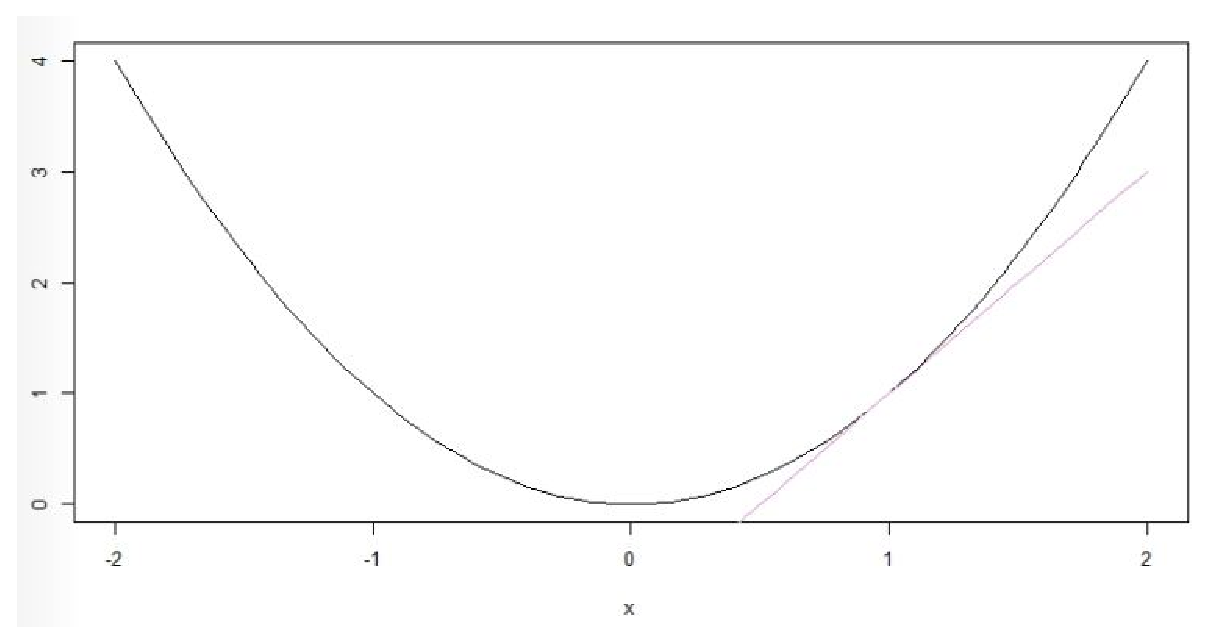
\includegraphics[scale = 0.5]{plsc43401_lec3_pic1}
\end{figure}

\end{frame}



\begin{frame}
\frametitle{Derivative Examples}

\begin{itemize}
\item[-] However, derivative may no exit. Let's see following canonical example. \pause Suppose $f(x) = |x|$ and consider $x_{0} = 0$.  Then, \pause 
\begin{eqnarray}
\lim_{x\rightarrow 0} R(x) & = & \lim_{x\rightarrow 0} \frac{ |x| } {x} \nonumber  \pause 
\end{eqnarray}
$\lim_{x \rightarrow 0^{-}} R(x) = -1$ \pause , but $\lim_{x \rightarrow 0^{+}} R(x) = 1$. \pause
\ \\So, $|x|$ not differentiable at $0$.

The figure looks like:

\end{itemize}

\end{frame}



\begin{frame}
\frametitle{Derivative Examples}

\begin{figure}[!ht]
\centering
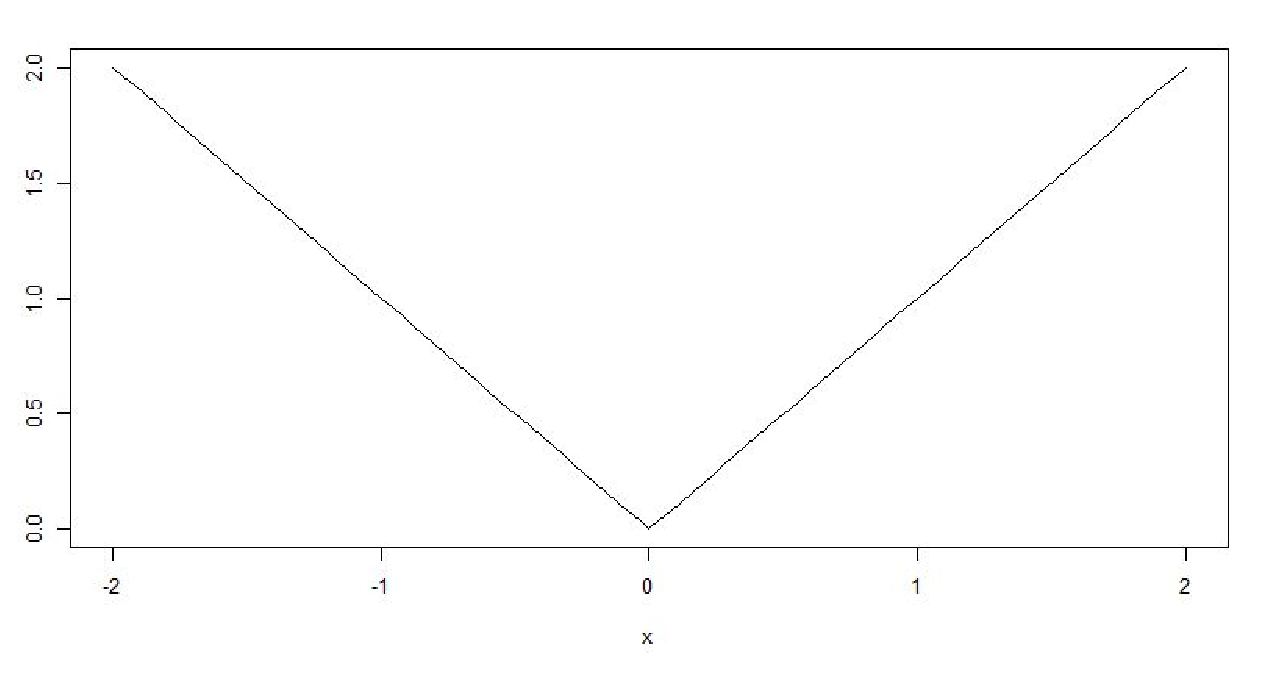
\includegraphics[scale = 0.5]{plsc43401_lec3_pic2}
\end{figure}

\end{frame}


\begin{frame}

\begin{itemize}
\item \textcolor{mygray}{Derivative}
\item \textcolor{myblack}{Derivative and Continuity}
\item \textcolor{mygray}{Derivative Rules}
\item \textcolor{mygray}{Mean Value Theorem}
\item \textcolor{mygray}{Second Derivatives}
\end{itemize}

\end{frame}



\begin{frame}
\frametitle{Derivative and Continuity}

Previous example that $|x|$ is continuous but not differentiable at 0 suggests that differentiability is a stronger condition than continuity. Then, a guess would be differentiability imply continuity.

\begin{thm} Let $f:\Re \rightarrow \Re$ be differentiable at $x_{0}$.  Then $f$ is continuous at $x_{0}$.
\end{thm} \pause

\end{frame}


\begin{frame}
\frametitle{Derivative and Continuity}

\begin{thm} Let $f:\Re \rightarrow \Re$ be differentiable at $x_{0}$.  Then $f$ is continuous at $x_{0}$.
\end{thm} \pause

\begin{proof}
Notice that, \pause 
\begin{eqnarray}
f(x) & = & \frac{ f(x) - f(x_{0})}{x- x_{0}} (x - x_{0} ) + f(x_{0} ) \nonumber \pause  \\
& = & R(x) (x - x_{0} ) + f(x_{0} ) \nonumber \pause 
	\end{eqnarray}
If $f(x)$ is continuous at $x_{0}$ then, $\lim_{x\rightarrow x_{0}} f(x) = f(x_{0})$. \pause 
\begin{eqnarray}
\lim_{x\rightarrow x_{0}} f(x) & = & \lim_{x\rightarrow x_{0} } [R(x) (x - x_{0} ) + f(x_{0}) ] \nonumber \\ \pause 
& = & \left(\lim_{x\rightarrow x_{0} } R(x) \right)\left(\lim_{x\rightarrow x_{0}} (x - x_{0}) \right)  + \lim_{x\rightarrow x_{0}} f(x_{0} ) \nonumber \\ \pause 
& = & f^{'}(x_{0} ) 0 + f(x_{0})  = f(x_{0} ) \nonumber
	\end{eqnarray}

\end{proof}

\end{frame}



\begin{frame}

\begin{itemize}
\item \textcolor{mygray}{Derivative}
\item \textcolor{mygray}{Derivative and Continuity}
\item \textcolor{myblack}{Derivative Rules}
\item \textcolor{mygray}{Mean Value Theorem}
\item \textcolor{mygray}{Second Derivatives}
\end{itemize}

\end{frame}



\begin{frame}
\frametitle{Useful Derivative Rules}

Suppose $a$ is some constant, $f(x)$ and $g(x)$ are functions \pause 
\begin{eqnarray}
f(x) = x & ; & f^{'}(x) = 1 \nonumber \\ \pause 
f(x) = a x^{k} & ; & f^{'}(x) = (a) (k) x ^{k-1} \nonumber \\ \pause 
f(x) = e^{x } & ; & f^{'} (x) = e^{x} \nonumber \\ \pause 
f(x) = \sin(x) & ; & f^{'} (x) = \cos (x) \nonumber \\ \pause 
f(x) = \cos(x) & ; & f^{'} (x) = - \sin(x) \nonumber 
\end{eqnarray}

\end{frame}



\begin{frame}
\frametitle{Derivative in Political Economy}

\begin{itemize}
\item The policy space is $\mathbb{R}$ \pause
\item A person (voter?)  has an ``ideal point" $p\in \mathbb{R}$ \pause
\item Person prefers policies that are closer to his/her ideal point: receives utility  from policy $x$ that is $u(x)=-|x-p|$ \pause
\item Since this isn't differentiable (and for other reasons), we may assume that 
\end{itemize}
$$u(x)=-(x-p)^2$$
$$u^\prime(x)=2p-2x$$

\end{frame}

\begin{frame}
\frametitle{Algebra of Derivatives}

\begin{thm} Suppose $f:\Re \rightarrow \Re$ and $g:\Re \rightarrow \Re$ and both are differentiable at $x_{0} \in \Re$.  Then, \pause 
\begin{itemize}
\item[i)] $h(x) = f(x) + g(x)$ is differentiable at $x_{0}$ and \pause 
\begin{eqnarray}
h^{'} (x_{0}) & = & f^{'}(x_{0}) + g^{'} (x_{0}) \nonumber \pause 
\end{eqnarray}
\item[ii)] $h(x) = f(x) g(x) $ is differentiable at $x_{0}$ and \pause 
\begin{eqnarray}
h^{'}(x_{0}) & = & f^{'}(x_{0}) g(x_{0}) + g^{'}(x_{0}) f(x_{0}) \nonumber  \pause 
\end{eqnarray}
\item[iii)] $h(x)  = \frac{f(x) }{g(x) }$ with $g(x) \neq 0$ then, \pause 
\begin{eqnarray}
h^{'}(x_{0}) & = &  \frac{f^{'}(x_{0}) g(x_{0}) - g^{'}(x_{0}) f(x_{0})} {g(x_{0})^2} \nonumber
\end{eqnarray}
\end{itemize}
\end{thm}

\end{frame}



\begin{frame}
\frametitle{Algebra of Derivatives: Examples}

\begin{itemize}
\item[1)] $f(x)= x^3 + 5 x^2  + 4 x$ \pause
\begin{eqnarray}
f'(x) & = & 3 x^2 + 5 * 2x + 4 \nonumber \pause \\
      & = & 3 x^2 + 10x + 4 \nonumber \pause
\end{eqnarray}
     
\end{itemize}

\begin{itemize}
\item[2)] $f(x) = sin(x) x^3$ \pause
\begin{eqnarray}
f'(x) & = & cos(X)  x^3 + sin(x)  3 x^2 \nonumber \pause \\
& = & cos(X)  x^3 + 3 sin(x)  x^2 \nonumber \pause
\end{eqnarray}
\end{itemize}

\begin{itemize}
\item[3)] $f(x) = \frac{e^{x} }{x^3}$ \pause
\begin{eqnarray}
f'(x) & = & \frac{e^{x}  x^{3} - e^{x}  3 x^{2} }{x^6} \nonumber \pause \\
& = & \frac{e^{x}  x^{3} - 3 e^{x} x^{2} }{x^6} \nonumber
\end{eqnarray}

\end{itemize}

\end{frame}



\begin{frame}
\frametitle{Chain Rule} 
Common to have functions in functions
\begin{eqnarray}
f(x) & = & \frac{e^{ - \frac{(x - \mu)^2}{2 \sigma^2}}}{\sqrt{2 \pi }  } \nonumber \\
		& = & \frac{f (g(x)) } {\sqrt{2 \pi}} \nonumber 
\end{eqnarray}

\ \\where $f(x) = e ^{- g(x)}$, $g(x) = \frac{(x - \mu)^2}{2 \sigma^2}$ \pause

To deal with this, we use the \alert{chain rule} \pause

\begin{thm} 
Suppose $g: \Re \rightarrow \Re$ and $f: \Re \rightarrow \Re$. Suppose both $f(x)$ and $g(x)$ are differentiable at $x_{0}$.  Define $h(x) = g(f(x))$.  Then, 
\begin{eqnarray}
h^{'}(x_{0}) & = & g^{'}(f(x_{0}))f^{'}(x_{0}) \nonumber 
\end{eqnarray}
\end{thm}

\end{frame}


\begin{frame}
\frametitle{Examples of Chain Rule}
\begin{itemize}
\item[-] $h(x) = e^{2x}$.  $g(x) = e^{x}$.  $f(x) = 2x$.  \pause So $h(x) = g(f(x)) = g(2x) = e^{2x}$.  Taking derivatives, we have \pause
\begin{eqnarray}
h^{'}(x) & = & g^{'}(f(x))f^{'}(x) = e^{2x}2 \nonumber 
\end{eqnarray} \pause
\item[-] $h(x) = \log(\cos(x) )$.  $g(x) = log(x)$.  $f(x) = \cos(x)$.  $h(x) = g(f(x)) = g( \cos(x)) = log(\cos(x))$  \pause
\begin{eqnarray}
h^{'}(x) & = & g^{'}(f(x))f^{'}(x) = \frac{-1}{\cos(x)} \sin(x) = -\tan (x) \nonumber 
\end{eqnarray}
\end{itemize}

\end{frame}



\begin{frame}

\begin{itemize}
\item \textcolor{mygray}{Derivative}
\item \textcolor{mygray}{Derivative and Continuity}
\item \textcolor{mygray}{Derivative Rules}
\item \textcolor{myblack}{Mean Value Theorem}
\item \textcolor{mygray}{Second Derivatives}
\end{itemize}

\end{frame}



\begin{frame}
\frametitle{Relative Maxima, Minima and Derivatives}

\begin{figure}[!ht]
\centering
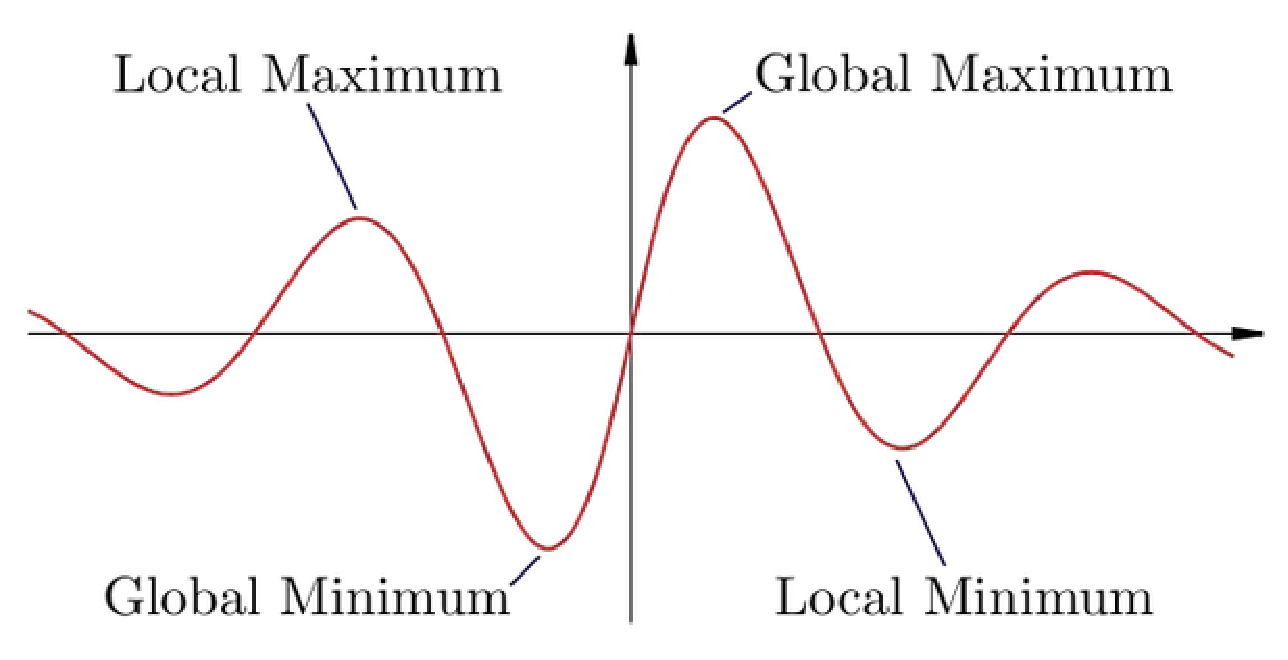
\includegraphics[scale = 0.36]{plsc43401_lec3_pic3}
\end{figure}

\begin{thm} Suppose $f:[a, b] \rightarrow \Re$.  Suppose $f$ has a relative maxima or minima on $(a,b)$ and call that $c \in (a, b)$.  Then $f^{'}(c) = 0$.  \end{thm}

\end{frame}



\begin{frame}
\frametitle{Relative Maxima, Minima and Derivatives}
\begin{thm} Rolle's Theorem Suppose $f:[a,b] \rightarrow \Re$ and $f$ is continuous on $[a,b]$ and differentiable on $(a,b)$.  Then if $f(a) = f(b) = 0$, there is $c \in (a, b)$ such that $f^{'}(c) = 0$.  \end{thm}

Proof
Intuition: Consider (WLOG) a relative maximum $c$. Consider the left-hand and right-hand limits
\begin{eqnarray}
\lim_{x \rightarrow c^{-}} \frac{f(x) - f(c) }{x - c } & \geq & 0 \nonumber \\
\lim_{x \rightarrow c^{+}} \frac{f(x) - f(c) } {x - c }  & \leq & 0 \nonumber 
\end{eqnarray}

\end{frame}


\begin{frame}
\begin{thm} Rolle's Theorem Suppose $f:[a,b] \rightarrow \Re$ and $f$ is continuous on $[a,b]$ and differentiable on $(a,b)$.  Then if $f(a) = f(b) = 0$, there is $c \in (a, b)$ such that $f^{'}(c) = 0$.  \end{thm}

But we also know that 
\begin{eqnarray}
\lim_{x \rightarrow c^{-}} \frac{f(x) - f(c ) }{x - c } & = & f^{'}(c) \nonumber \\
\lim_{x \rightarrow c^{+}} \frac{f(x) - f(c) } {x - c }  &  =  & f^{'}(c)  \nonumber 
\end{eqnarray}

The only way, then, that \\
$\lim_{x \rightarrow c^{-}} \frac{f(x) - f(c) }{x -c}  = \lim_{x \rightarrow c^{+}} \frac{f(x) - f(c) } {x - c} $ is if $f^{'}(c) = 0$.  

\end{frame}



\begin{frame}
\frametitle{Mean Value Theorem} 

\begin{thm} If $f:[a,b] \rightarrow \Re$ is continuous on $[a,b]$ and differentiable on $(a,b)$, then there is a $c \in (a,b)$ such that 

\begin{eqnarray}
f^{'}(c) & = & \frac{f(b) - f(a) } { b - a} \nonumber 
\end{eqnarray}
\end{thm}

\end{frame}



\begin{frame}

\begin{itemize}
\item \textcolor{mygray}{Derivative}
\item \textcolor{mygray}{Derivative and Continuity}
\item \textcolor{mygray}{Derivative Rules}
\item \textcolor{mygray}{Mean Value Theorem}
\item \textcolor{myblack}{Second Derivatives}
\end{itemize}

\end{frame}



\begin{frame}
\frametitle{Second Derivatives}

Now, we can extend our definition of derivatives to higher order derivative. Let's first consider second order derivative.

\frametitle{Second Derivatives}

\begin{defn} Suppose $f:\Re \rightarrow \Re$ is differentiable.  Recall we write this as $f^{'}$ and suppose that $f^{'}:\Re \rightarrow \Re$.  Then if the limit, 
\begin{eqnarray}
\lim_{x\rightarrow x_{0} } R(x) & = & \frac{f^{'}(x) - f^{'}(x_{0} ) } {x - x_{0} } \nonumber 
\end{eqnarray}
exists, we call this the \alert{second derivative} at $x_{0}, f^{''}(x_{0})$.  
\end{defn}

\end{frame}


\begin{frame}
\frametitle{Second Derivatives}

\ \\Now, let's see a figure of second derivative.

\begin{figure}[!ht]
\centering
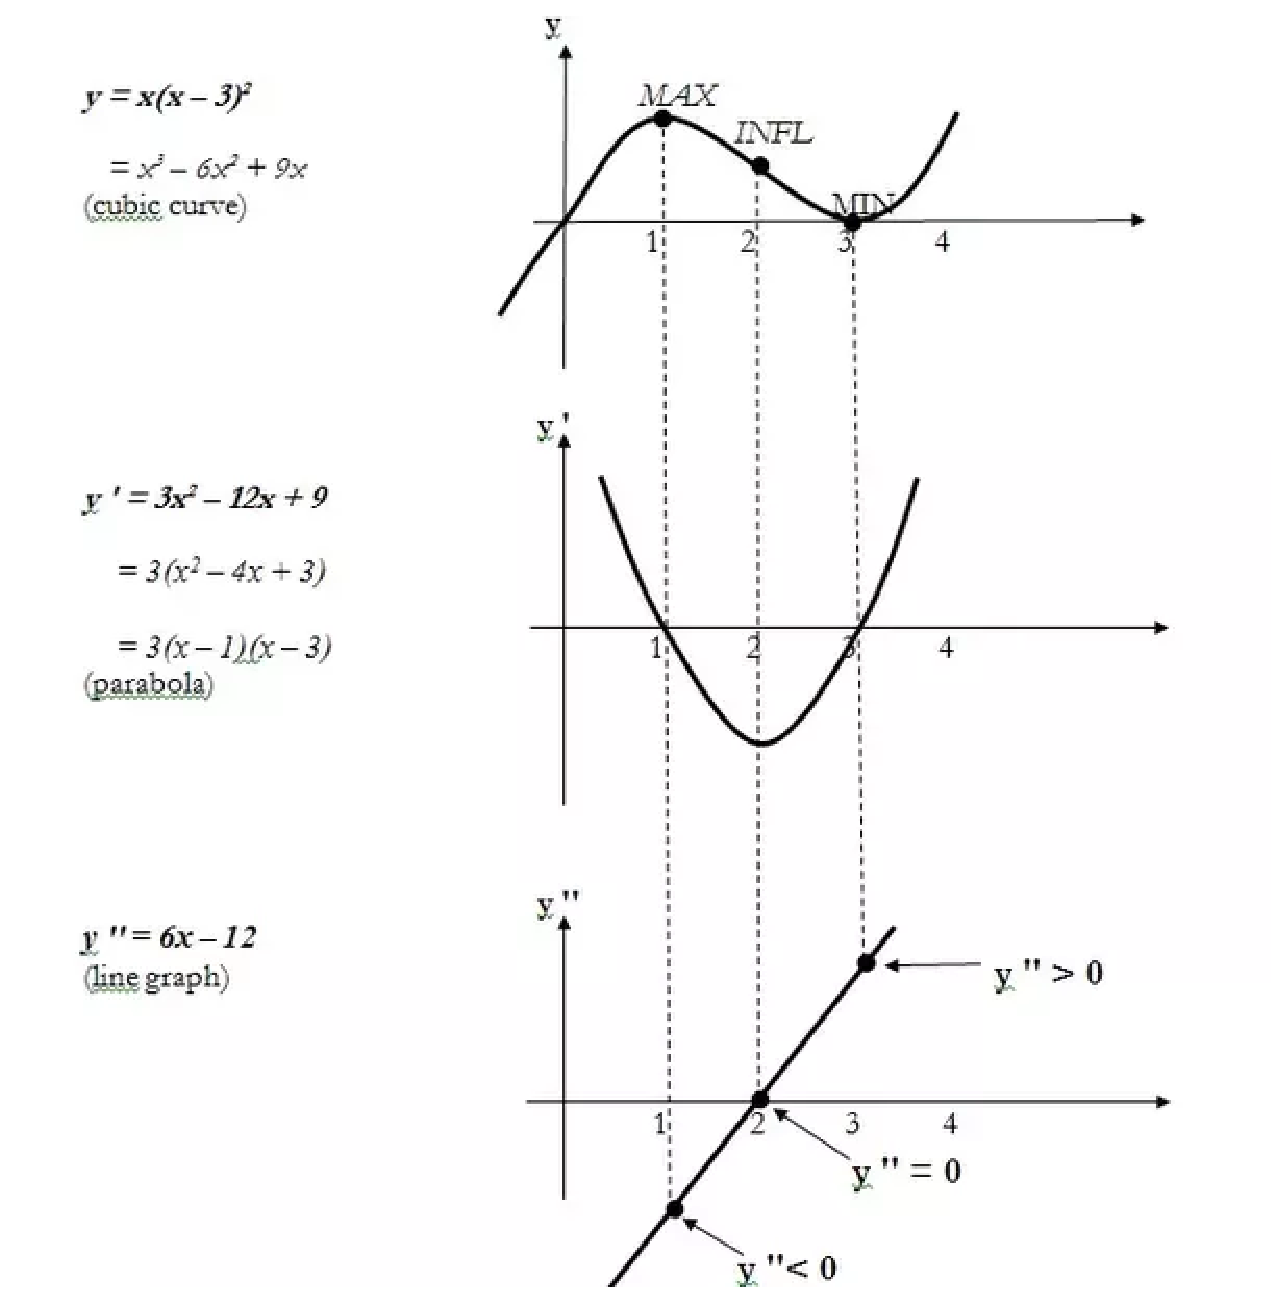
\includegraphics[scale = 0.3]{plsc43401_lec3_pic4}
\end{figure}

\end{frame}


\begin{frame}
\frametitle{Example of Second Derivatives}

\only<1>{\begin{eqnarray}
f(x) & = & x \nonumber \\
f^{'}(x) & = & 1 \nonumber \\
f^{''} (x) & = & 0 \nonumber 
\end{eqnarray}}


\only<2>{\begin{eqnarray}
f(x) & = & e^{x} \nonumber \\
f^{'}(x) & = & e^{x} \nonumber \\
f^{''}(x) & = & e^{x} \nonumber
\end{eqnarray}}

\only<3>{
\begin{eqnarray}
f(x) & = & \log (x) \nonumber \\
f^{'}(x) & = & \frac{1}{x} \nonumber \\
f^{''}(x) & = & \frac{-1}{x^2} \nonumber 
\end{eqnarray}
}

\only<4>{\begin{eqnarray}
f(x) & = & \frac{1}{x} \nonumber \\
f^{'}(x) & = & \frac{-1}{x^2} \nonumber \\
f^{''}(x) & = & \frac{2}{x^3} \nonumber 
\end{eqnarray}}


\only<5>{\begin{eqnarray}
f(x) & = & -x^2 + 20 \nonumber \\
f^{'}(x) & = & -2 x  \nonumber \\
f^{''}(x) & =& - 2 \nonumber 
\end{eqnarray}}



\end{frame}


\end{document}
